\appendix

\section{Prompt, Skeleton Example and Additional Results}
\label{app:details}

Listing~\ref{lst:prompt} gives the prompt template of condition C0 (Section~\ref{sec:method}), Table~\ref{tab:skeleton} illustrates the skeleton extraction of Section~\ref{sec:metric1}, Fig.~\ref{fig:dist} and Fig.~\ref{fig:domain} show the distribution of skeleton cosine in C0 overall and per project, Table~\ref{tab:sweep} gives the threshold sensitivity analysis of Section~\ref{sec:res-b3}, and Table~\ref{tab:rq2} gives the parser results of RQ2.

\begin{lstlisting}[caption={Prompt template of condition C0. Braced placeholders are instantiated by project at run time.},label={lst:prompt}]
System: {domain_specific_system_message}
User:
Generate a BDD Gherkin file for the following user story.
Follow the exact style, wording, and conventions shown in the Example.

EXAMPLE USER STORY:
{example_user_story_from_same_domain}

EXAMPLE GHERKIN:
{example_gherkin_from_same_domain}

---
NOW GENERATE FOR THIS USER STORY:
{user_story_text}
\end{lstlisting}

\begin{table}[t]
\centering
\caption{Skeleton extraction on a short Sylius-style fragment.}
\label{tab:skeleton}
\scriptsize
\begin{tabular}{ll}
\hline
Original line & Skeleton line\\
\hline
\texttt{@ui} & (removed)\\
\texttt{Given a product "T-Shirt" priced at "\$20.00"} & \texttt{Given a product <PARAM> priced at <PARAM>}\\
\texttt{When I add 3 units to the cart} & \texttt{When I add <NUM> units to the cart}\\
\texttt{| name | price |} & (removed)\\
\texttt{Then the total should be "\$60.00"} & \texttt{Then the total should be <PARAM>}\\
\hline
\end{tabular}
\end{table}

\begin{figure}[t]
\centering
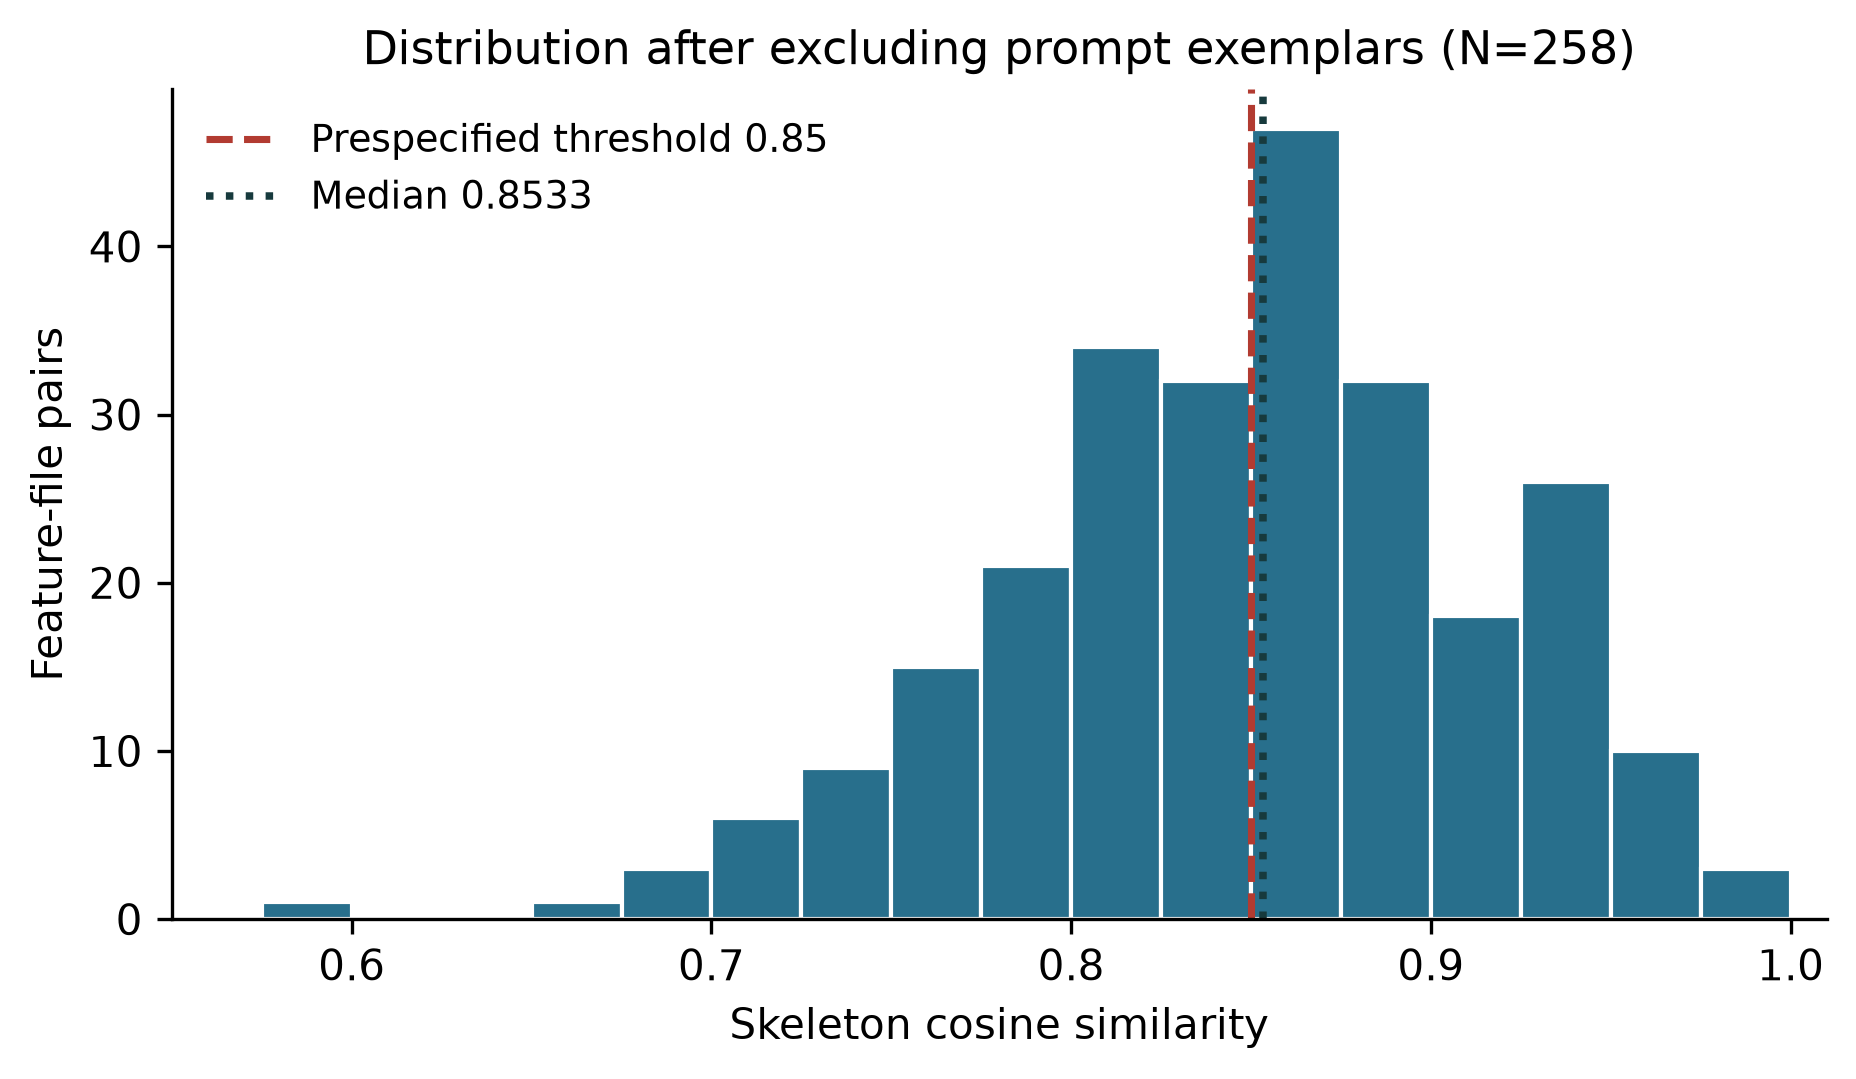
\includegraphics[width=0.72\textwidth]{figures/fig1_skeleton_distribution_258.png}
\caption{Distribution of skeleton cosine similarity for the 258 non-exemplar files (condition C0).}
\label{fig:dist}
\end{figure}

\begin{figure}[t]
\centering
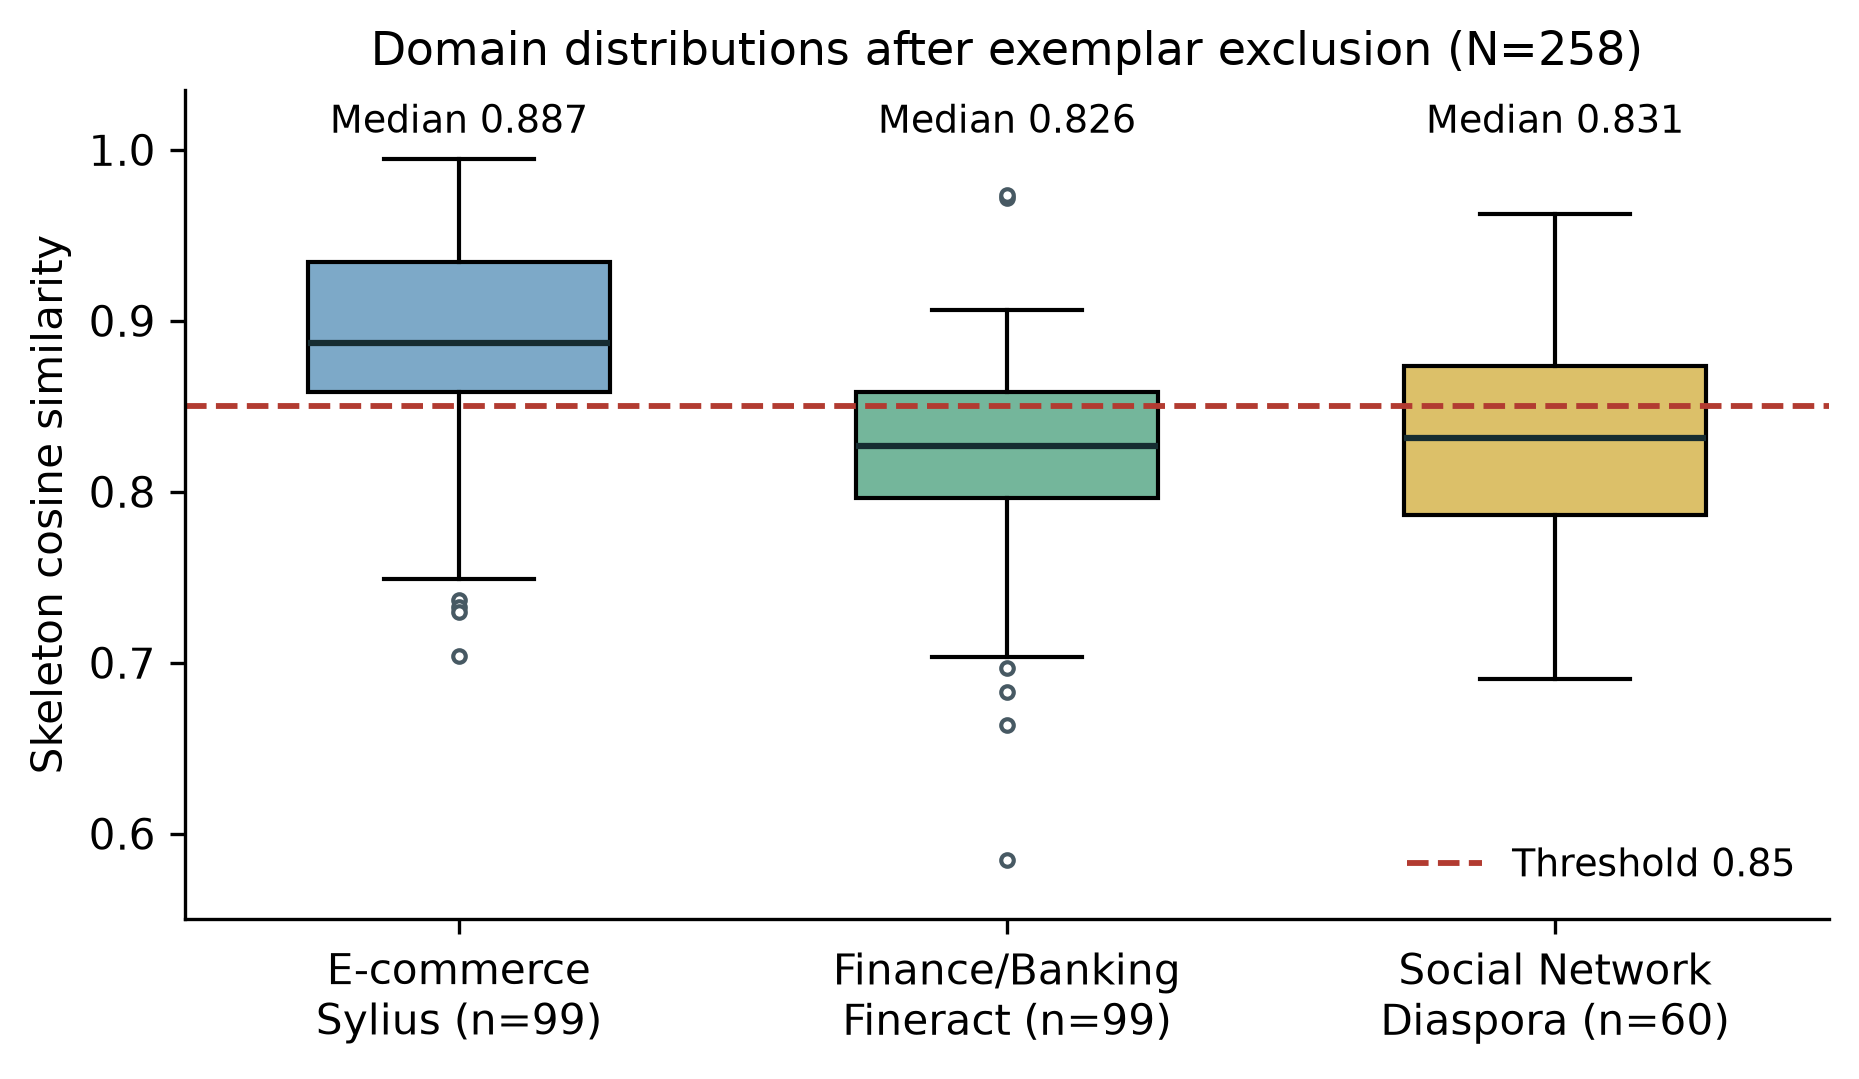
\includegraphics[width=0.72\textwidth]{figures/fig2_domain_distributions_258.png}
\caption{Skeleton cosine similarity per project (C0, $N = 258$). The dashed line marks 0.85.}
\label{fig:domain}
\end{figure}

\begin{table}[t]
\centering
\caption{Threshold sensitivity (C0, $N = 258$). The $p$-value is the one-sided Wilcoxon test that the median exceeds $t$.}
\label{tab:sweep}
\begin{tabular}{rrrrrrr}
\hline
$t$ & Share $\ge t$ [95\% CI] & Median $- t$ & $p$ & Sylius & Fineract & Diaspora\\
\hline
0.80 & 78.3\% [72.8, 83.2] & $+0.053$ & $< 0.001$ & 91.9\% & 73.7\% & 63.3\%\\
0.82 & 67.8\% [61.8, 73.5] & $+0.033$ & $< 0.001$ & 87.9\% & 56.6\% & 53.3\%\\
0.84 & 59.3\% [53.0, 65.4] & $+0.013$ & 0.010 & 84.8\% & 40.4\% & 48.3\%\\
0.85 & 52.7\% [46.4, 58.9] & $+0.003$ & 0.474 & 77.8\% & 34.3\% & 41.7\%\\
0.86 & 43.4\% [37.3, 49.7] & $-0.007$ & 0.988 & 73.7\% & 22.2\% & 28.3\%\\
0.88 & 30.6\% [25.1, 36.6] & $-0.027$ & 1.000 & 55.6\% & 12.1\% & 20.0\%\\
0.90 & 22.1\% [17.2, 27.7] & $-0.047$ & 1.000 & 45.5\% & 4.0\% & 13.3\%\\
\hline
\end{tabular}
\end{table}

\begin{table}[t]
\centering
\caption{Parser compliance of condition C0 (behave 1.3.3 parser).}
\label{tab:rq2}
\begin{tabular}{lrr}
\hline
Statistic & $N = 258$ (primary) & $N = 261$\\
\hline
Parser PASS / FAIL & 255 / 3 & 258 / 3\\
ESR & 98.84\% & 98.85\%\\
95\% Clopper--Pearson CI & [96.64\%, 99.76\%] & [96.68\%, 99.76\%]\\
Exact binomial $p$ ($p_0 = 0.80$) & $4.6 \times 10^{-21}$ & $2.4 \times 10^{-21}$\\
\hline
\end{tabular}
\end{table}

\clearpage
\section{Perturbation Test}
\label{app:perturb}

\textbf{Design.} The perturbation test measured whether the metric reacts to seeded defects. From the reference files, 120 scenarios (40 per project, fixed seed) were extracted, and eight operators were applied where applicable: changing a number, a quoted value, a comparison operator or a negation, dropping a Then or a Given step, swapping a When with a Then, and moving a Then to the front. Each mutant was compared with its original scenario using the same skeleton metric.

\textbf{Results.} The 120 extracted scenarios yielded 683 applicable mutants. Of these, 29 mutants do not parse, and the extraction omitted the Background of 74 of the 120 source scenarios. Restricting to the 623 pairs in which both texts parse and the original has no keyword-order flag, every mutant keeps a skeleton cosine of at least 0.8995 with its original. At 0.90, 622 of 623 mutants would still pass, and at 0.95, 97.9\%. For changed numbers and quoted values (179 pairs) the skeletons are identical, which follows from masking and is not an empirical finding. Swapped When/Then steps and Then steps moved to the front (210 pairs) score at least 0.954, although the keyword-order check flags all of them. Because the test compares single scenarios and the main metric compares whole files, these results show insensitivity at the scenario level and do not estimate a false-negative rate for whole files.
